\chapter{Feed 流优化验证}

\section{预渲染优化验证}

只通过示例无法很好地对优化结果进行验证,同时目前还没有一个能够量化的流畅性指标来证明优化的程度。因此需要搭建一个相对真实的视频 Feed 流场景,并在此基础上建立准确、能够量化的流畅性指标来验证预渲染优化对流畅性体验的提升。

\subsection{搭建视频 Feed 流场景}

视频 Feed 流选用 RecyclerView 搭建,播放器选用谷歌的 Media 库,通过自定义视频展现的 View 来获取视频画面并播放。该案例中,通过解析本地文件夹中的视频,将它们平铺在列表中形成视频 Feed 流。用户上下滑动屏幕,即可与刷短视频一样浏览文件夹中的视频。同时,为了真实模拟短视频应用的体验,开发了沉浸式背景取色、松手起播、视频首帧图像作为视频封面等模块,让整体的体验更加像市面上的短视频应用。

接下来是验证优化结果的过程。为了引入卡顿,在视频卡片的 ViewHolder 绑定过程中人为引入一段耗时逻辑来模拟卡片进行数据绑定时的耗时操作。将视频 Feed 流的 LayoutManager 替换为引入了预渲染机制的版本,同时开启不同的模式来体验。引入的耗时逻辑越耗时,优化的体验就越明显。具体表现为:在没有预渲染的情况下,每一次滑动都会产生明显的卡顿,并且上滑的动画也出现了不同程度的调帧;在一直预渲染的模式下,只有第一次滑动是流畅的,其它的时候由于额外布局空间一直存在,滑动依然会产生卡顿;在滚动停止触发预渲染的模式下,只有滚动停止时才会进行预渲染,每一次滚动的流畅性都大大增加;在外界触发预渲染的情况下,只有视频开始播放并且滚动已经停止时才会触发预渲染。这意味着只要用户在视频播放之后才滑动屏幕,预渲染的卡片就一直存在,并且预渲染的逻辑也能够避开是视频起播的流程,最大程度地分散耗时任务的布局。

\subsection{Android 绘制体系的调研}

想要获得准确的流畅性指标,需要对 Android 应用绘制的流程以及其底层的刷新原理非常了解,因此对于这部分内容进行了调研。通过阅读 Android Framework 层和刷新相关的部分源码,总结出了与流畅性相关的绘制流程。

Android 系统底层采用 Skia,OpenGL 等引擎进行绘制,而在上层封装好的组件就是 Canvas 和 View \cite{tahir2013learning}。View绘制系统是 Android 开发者最常用到的 UI 编写 API,同时各种动画、自定义样式等绘制操作也都是交由 View 和 Canvas 来完成。

本课题用到的优化机制,主要是针对 View 的,因此这里着重介绍一下 View 的绘制流程。在 Android 应用中,View 占据了一块屏幕上的矩形区域。在这个区域内,UI 将被显示给用户,同时这块区域也负责处理用户、应用本身输入的事件,从而和用户进行交互\cite{aljarrah2016maintaining}。View 的体系非常庞大,绘制系统也非常复杂。这里主要针对 View 的大致分类和普通 View 的绘制流程进行说明。

\subsubsection*{View 的分类}

从总体的功能上看,View 只分为两种:普通的 View 以及 ViewGroup。顾名思义,ViewGroup是用来承载其它 View 和 ViewGroup 的容器;而普通的 View 无法承载其它的 View,只能作为直接和用户交互的组件。在 Android 系统中,View 体系通过树形结构来存储,因此,这棵树上所有的非叶子节点都是 ViewGroup,所有的叶子节点都是普通的 View。

从代码层面来看,ViewGroup 继承自 View,因此 ViewGroup 有着和普通的 View 相似的行为,也需要进行绘制和布局等流程。只不过,ViewGroup 更加关心的是自己内部的子 View 的测量流程,对它们进行统一的管理。\

从内容层级来看,Android 应用程序从最顶层的 DecorView 出发(DecorView 本身被 ViewRootImpl 持有),到持有内容的容器 contentParent,最后到应用开发者主动向 Window 中添加的各种 View,如图 4.1。这些系统级别的 View 一部分是为了管理系统的应用以及悬浮窗等 Window 的通用行为,另一部分是为了给开发者提供额外的扩展能力。因此,对于 View 的性能进行优化主要也是开发者自行添加的这一部分。

% View 层级的图

\begin{figure}
    \centering
    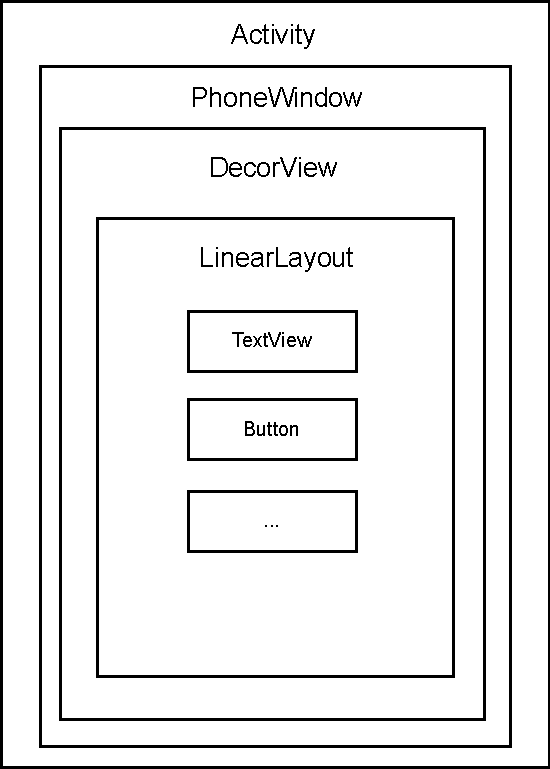
\includegraphics[scale=0.7]{assets/view-hierarchy.pdf}
    \caption{Android 应用程序的 View 层级}
\end{figure}

\subsubsection*{Android 屏幕刷新原理}

在 Android 系统中,屏幕的显示操作需要靠三个部分来完成:CPU,GPU 和显示器。其中,CPU 负责进行绘制信息的计算,其中就包括之前介绍的 View 的绘制流程。这些计算好的信息会交给 GPU 进行图形渲染,生成每一个屏幕像素点的颜色信息,并存储到一个缓存当中。当需要让显示器进行显示时,GPU 和显示器的缓存会进行交换,这样显示器得到的就是新的要显示的内容。下面针对屏幕刷新的情况介绍一些概念:

\begin{itemize}
    \item 屏幕刷新率:一秒内屏幕刷新的次数。由于显示器拿到的每一个缓存都包含了屏幕上所有要更新的信息,因此屏幕的显示模式是在固定的时间将屏幕上的所有像素点进行更新。不过某些情况下,如果前后两次的像素是一致的,那么可以选择不更新,这个操作取决于显示器。因此,即使提高了 GPU 将像素信息传送到显示器的速度,屏幕刷新率也是不变的,因为这个指标是对于显示器性能的衡量,而非实际情况;
    \item 逐行扫描:显示器显示像素的原理并不是一次性将缓存中所有的像素点真正更新到屏幕上,而是逐行进行扫描\cite{张春明2002显示器刷新率的测试以及逐行显示器的辨别方法}。因此,这段扫描的时间决定了显示器的素质。通常情况下, Android 手机的显示器扫描一次整个屏幕需要约16.67毫秒。因此,这个时间的结果就是屏幕每秒钟刷新的次数约为60次,也就是屏幕刷新率为60Hz;
    \item 帧率:与屏幕刷新率相对的,帧率表示实际情况下将画面传送给显示器的速度。对于运行在 Android 系统的 CPU 来说,这个过程交给了应用的主线程。因此,如果主线程在执行任务的时候过于耗时,没能及时将数据传递给 GPU 和显示器,那么就会让这一帧无法显示在屏幕上,导致屏幕上显示的还是原来的像素,这就是卡顿产生的原因。因此,为了保证真实的帧率能够贴近屏幕刷新率,Android 应用的主线程在处理任务时应该尽可能快,这样才能保证所有的绘制操作顺利进行并最终显示在屏幕上。
\end{itemize}

在某些情况下,屏幕的显示可能会产生抖动。产生这种现象的原因是,当显示器读取缓存,并显示到屏幕上时,GPU 正在向缓存中写入数据。由于并没有做读写保护,所以前后的像素点并不是来自于同一帧。因此后果就是屏幕上的画面产生了撕裂感\cite{yun2017reducing}。解决这种问题的方法是使用双缓存。也就是 GPU 写入的缓存,和显示器读取的缓存并不是同一个。GPU 只写入 Back Buffer,显示器只读取 Frame Buffer。而到了需要刷新的时机时,两个缓存的引用会进行交换。由于这个交换的过程非常快,因此可以杜绝绝大部分的画面撕裂问题。

然而,在目前的双缓存机制下,卡顿的问题还是无法很好地解决。当 CPU(或者 GPU)在当前帧的持续时间内,无法及时完成图像信息的计算,那么就会发生卡顿。在这种情况下会发现无论是 CPU 还是 GPU,都无法使用 Frame Buffer 或者 Back Buffer。因为前者需要被显示器读取来维持卡顿的帧;后者的数据还没有被显示器读取,等到卡顿帧结束之后,它们还需要被显示到屏幕上。这就导致如果在这个过程中 CPU 和 GPU 有计算任务,计算的结果没有地方保存,也就浪费了 CPU 和 GPU 的绘制时间。针对这个问题,Android 引入了三缓存(Triple Buffering)机制\cite{egilmez2017user}。在三缓存机制下,有两个 Back Buffer 存在,当其中一个因为卡顿而被占用时,CPU 和 GPU 的计算结果就可以存储到另一个缓存中。这样就能有效减少卡顿的传递性带来的连续卡顿。

下一个问题是两个缓存进行交换的时机。如果无法保证交换时的读写安全,那么依然会产生显示上的问题。当屏幕的最后一个像素显示完毕后,设备需要一段空闲时间,以便将指针移动回第一个像素来显示下一帧的内容。这段空闲的时间叫做 Vertical Blanking Interval(VBI)\cite{anderson1971vertical}。在这段时间内,屏幕上的内容依然会保持原状,并且显示器也不会去读缓存中的内容。因此,这个时间就是进行缓存交换的最佳时刻。在VBI的时间内,系统会发射出用于同步时钟信号的垂直脉冲。这个垂直脉冲也就是 VSync 信号,是判断一帧到达的关键信息。

\subsubsection*{Choreographer 和屏幕信号进行同步}

以上的介绍很大程度上是在硬件层面描述 Android 系统中应用的刷新模式。下面从软件层面来说明这一过程,来看看在 Android 系统中,画面的刷新流程到底是怎样的。对于应用层的进程来讲,其和屏幕刷新相关的主要媒介是通过一个上层的 Framework 组件 —— Choreographer。

Choreographer 的职责是协调动画、用户输入事件(触摸,外接鼠标等)和绘制流程。它通过底层注册的驱动程序接受系统发出的时间脉冲(也就是上文提到的 VSync 信号),来组织下一帧应该绘制的信息。其中包括让 CPU 去处理下一帧的图像信息,也包括将这些计算好的信息提交给 GPU 来进行渲染。接下来提到的 View 的绘制以及其对于用户输入事件的处理也都是由 Choreographer 在每一帧发起的。

接下来介绍 Choreographer 具体的工作流程。通过之前对于 Android 消息机制的介绍可知,在 Android 应用中,每一个应用的主进程在启动时,都会开启一个 Looper,应用程序的其它组件通过 Handler 向该 Looper 发送消息。显然,主线程对应的 Looper 就是主要用来处理各种绘制操作,而绑定了该 Looper 的 Handler 用来向主线程提交各种类型的绘制操作任务。对于 Choreographer,当接收到底层发送的 VSync 信号时,就会向主线程提交一个这样的绘制任务。这就是 Android 应用程序中各种动态界面绘制的源头。

% 这个 Looper 的运行函数是一个无限循环,在每一次循环中,会从消息队列中取出一条消息执行,并不断重复这个过程。向 Looper 提供一条消息的方式就是通过另一个组件 —— Handler。Handler 可以发送各种类型的消息,同时具备延时功能。发送的消息会被添加到等待队列中,等待 Looper 将其取出并执行。

因为这样的绘制机制,开发者在开发以及优化应用时,无需关心每一个 VSync 信号实际被发出的时间,只需要关心注册的监听器什么时候能接收到 VSync 信号。在这个信号到来时执行绘制的行为,并争取在下一个 VSync 信号到来之前完成它。因此,需要区分“帧”和“绘制行为”的区别。通常所说的帧指的是每两个 VSync 信号的间隔时间。这段时间内,绘制行为有可能完成,也有可能没有完成;而绘制行为指的是由 Choreographer 发起的从 CPU 到 GPU 最后到显示器的一系列操作。这一串行为在正常情况下只能在一个 VSync 信号到来时开始执行,并在下一个 VSync 信号到来前执行完毕。如果没有及时完成绘制行为,那么下一帧依旧只能显示上一帧的内容,直到绘制完成,缓存可用为止。了解了这些,能够帮助开发者在收集流畅性指标时,制定更加精确的收集方案。

Choreographer 在一帧内所做的绘制工作主要有:

\begin{itemize}
    \item 处理用户输入事件;
    \item 处理动画;
    \item 处理 View 的绘制流程。
\end{itemize}

这些绘制工作都作用在应用的 View 树上,通过遍历 View 层级中的各个 View 来对其进行重新绘制,相应触摸之后的新行为等等。在这个过程中,也涉及到很多的性能优化过程,比如增量更新以及脏区计算等等。因此,对于这部分逻辑的改动需要格外小心,确保在优化完毕后,View 的行为对于业务来说和优化之前保持一致。

\subsection{流畅性指标建设}

能够量化的最直观的流畅性指标就是当前的实时帧率(FPS)。而实时帧率的计算是从 Android 屏幕刷新的过程以及 Choreographer 进行绘制流程得到的。在 API 24 之后,谷歌官方给出了统一的绘制帧情况的收集方法,通过注册 Window 的 onFrameMetricsAvailable() 回调,能够得到绘制的每一帧的信息。通过这些信息能够计算当前绘制行为持续的时间等情况,从而计算出帧率和其它的指标。在本案例中,计算的指标为长帧占比,即绘制时长超过两个 VSync 间隔的绘制行为在所有绘制行为中的比率。这个指标能够反映当前时间内绘制的流畅程度,长帧占比越高,卡顿的现象就更加严重。

在预渲染关闭和开启的情况下分别统计滑动完所有视频过程中的长帧占比,并控制不同的视频数量,得到如图 4.2 的结果。
    
\begin{figure}[H]
	\centering
		\begin{tikzpicture}
			\begin{axis}[
				xlabel={视频数量(个)},
				ylabel={长帧占比(百分比)},
				xmin=2, xmax=10,
				ymin=8, ymax=18,
				xtick={2, 3, 4, 5, 6, 7, 8, 9, 10},
				ytick={8, 9, 10, 11, 12, 13, 14, 15, 16, 17, 18},
				legend pos=outer north east,
				grid style=dashed,
			]
			
			\addplot[
				color=black,
				mark=square
				]
				coordinates {
				(2,11.11)(3,11.76)(4,14.28)(5,16)(6,17.24)(7,17.14)(8,17.07)(9,17.39)(10,17.3)
				};
			\addlegendentry{预渲染关闭}
		
			\addplot[
				color=black,
				mark=star
				]
				coordinates {
				(2,11.11)(3,11.11)(4,11.11)(5,13.79)(6,14.7)(7,15.38)(8,15.9)(9,15.38)(10,12.67)
				};
			\addlegendentry{一直预渲染}
		
			\addplot[
				color=black,
				mark=diamond
				]
				coordinates {
				(2,8.69)(3,8.51)(4,8.57)(5,8.6)(6,8.62)(7,8.63)(8,8.64)(9,8.64)(10,8.13)
				};
			\addlegendentry{滚动停止预渲染}
		
			\addplot[
				color=black,
				mark=oplus
				]
				coordinates {
				(2,8.33)(3,8.88)(4,8.95)(5,8.98)(6,8.92)(7,8.95)(8,8.97)(9,8.98)(10,8.41)
				};
			\addlegendentry{外界触发预渲染}
			
			\end{axis}
		\end{tikzpicture}
	\caption{流畅性指标折线图}
\end{figure}

在预渲染关闭的情况下,由于每一个视频都需要在滑动的时候进行耗时的数据绑定,因此长帧占比迅速提升到一个平均值并在周围波动;在一直预渲染的情况下,只有滑动到最后一个是视频时,由于不需要预渲染,所以长帧占比大幅度降低,但总体情况依然不理想;在滚动停止预渲染和外界预渲染的情况下,数据绑定不会在滑动的时机进行,所以滑动时的长帧占比大幅度降低。反映到体验上就是用户的滑动会感觉更加流畅。

\section{异步创建优化验证}

为了验证异步创建 View 优化的效果,搭建了一个类似新闻页面的 RecyclerView。此页面在首次刷新时会进行一次假的网络请求,在一段时间之后会返回一些新闻数据,同时用于 Adapter 进行数据绑定并通知 RecyclerView 进行布局。为了模拟 View 创建过程中的耗时行为,人为在子 View 的构造方法中引入耗时逻辑。在这个过程中,开启异步预加载和关闭预加载的情况下,可以明显感觉到有异步创建的时候加载的速度更快。为了进一步量化优化效果,设计了一个“秒开检测框架”:当 RecyclerView 首次刷新时,通过 ViewTreeObserver 的监听器捕获事件,并在回调方法中执行检测逻辑。

\begin{figure}[H]
    \centering
    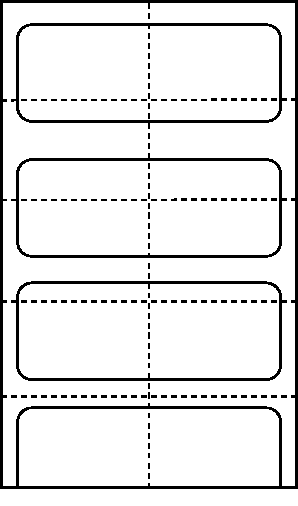
\includegraphics{assets/visibility-check.pdf}
    \caption{秒开检测框架的应用实例}
\end{figure}

秒开框架的检测思路如图 4.3:将屏幕分成若干个目标区域,每个区域通过左上角顶点的坐标,以及区域的长和宽来唯一标识。当进行检测时,扫描检测范围内所有的 View,让业务方来决定有效区域的大小。这里的有效区域是指对用户来说有意义的区域大小。以文本类 TextView 来举例子,有效区域就是真实文本所覆盖的区域,不包括四周的留白。当有效区域和屏幕的目标区域的交集超过了一定阈值时,该目标区域被标记为有效;当所有(或大部分)的目标区域都被认为有效时,此时的时间戳与页面开始刷新的时间戳之差为页面首次刷新的时长,即首帧时长。该时长标志着应用加载的速度,给用户带来流畅性的体感。时间越短表明对用户来说刷新的感知时间越短,体验越好。

\begin{figure}[H]
    \centering
    \begin{tikzpicture}
        \begin{axis}[
            ybar, % 使用柱状图样式
            width=13cm,
            scale=0.8,
            enlarge x limits={abs=0.5}, % 扩大 X 轴范围,确保边缘数据点完全显示
            ylabel={首刷时长(秒)}, % Y轴标签
            xlabel={缓存容量(个)},
            xmin=0, xmax=15, % X轴范围
            ymin=0, ymax=6, % Y轴范围
            xtick={0,1,...,15}, % X轴刻度
            ytick={0,0.5,...,6}, % Y轴刻度
            nodes near coords, % 在柱状图上显示具体数值
            nodes near coords align={vertical}, % 数值显示垂直方向
            every node near coord/.append style={font=\tiny, inner ysep=3pt} % 设置文字样式和距离
            ]
            \addplot[fill=blue!0] coordinates {
                (0, 5.17)(1, 5.17)(2, 5.33)(3, 4.51)(4, 4.44)(5, 4.3)
                (6, 4.06)(7, 3.83)(8, 3.59)(9, 3.38)(10, 3.16)(11, 3.52)
                (12, 3.51)(13, 3.93)(14, 4.33)(15, 4.74)
            }; % 添加柱状图数据,x=0,y=3.5
        \end{axis}
    \end{tikzpicture}
    \caption{首刷时长与缓存个数的关系}
\end{figure}



当没有异步创建(缓存容量为0),以及有异步创建的情况下缓存容量逐渐增加的过程中,缓存容量与首帧时长的关系如图 4.4。可以发现,随着缓存容量不断扩大,能够提前预加载的 View 也不断变多,所以首刷时长会不断降低;但由于屏幕大小的限制,缓存数量也不是越多越好。当缓存个数超出屏幕能承载的最多 View 个数时,多出来的部分反而会让首次刷新变得更慢。所以需要针对具体的业务场景找到一个最佳的缓存池容量来实现最佳的首刷时长优化。